\documentclass[crop,tikz]{standalone}
\usepackage{amsmath}

\usetikzlibrary{positioning,arrows,shapes}
\usetikzlibrary{decorations.pathmorphing}
\usetikzlibrary{decorations.markings}

\begin{document}
  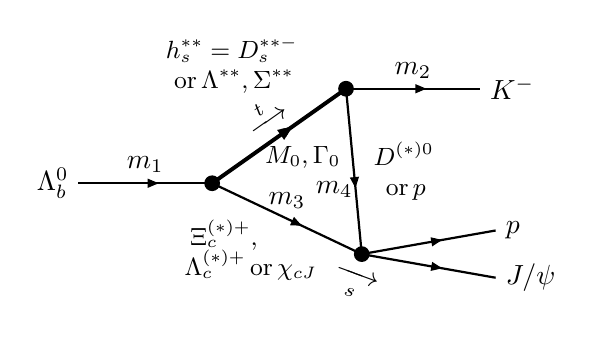
\begin{tikzpicture}[node distance=1.2cm and 1.7cm,
    scalar/.style={thick,draw=black, postaction={decorate},
      decoration={markings,mark=at position .6 with {\arrow[black,scale=0.5]{triangle 45}}}}]

    % Set coordinates
    \coordinate[] (a1);
    \coordinate[right=of a1] (a2); \coordinate[above right=of a2]
    (b1);
    \coordinate[below right=of a2, xshift=2mm, yshift=3mm] (b2);
    \coordinate[right=of b1] (c1);
    \coordinate[right=of b2, yshift=3mm] (c2);
    \coordinate[right=of b2, yshift=-3mm] (c3);

    % Draw lines
    \node[left] (a1) {$\Lambda_b^{0}$};
    \draw[scalar] (a1) -- node[above] {$m_1$} (a2);
    \draw[scalar] (a2) -- node[below,xshift=3mm] {\small $M_0,\Gamma_0$}
                          node[xshift=-6mm,yshift=9mm] {\parbox{2cm}{\centering\small $h_s^{**}=D_s^{**-}$\\$\text{\,or\,}\Lambda^{**}, \Sigma^{**}$}} (b1);
    \draw[scalar, line width=0.5mm] (a2) -- node[above,sloped] {$\xrightarrow[]{\hspace{1mm}t\hspace{1mm}}$} (b1);
    \draw[scalar] (a2) -- node[xshift=-8mm,yshift=-4mm] {\parbox{1cm}{\centering\small$\Xi_c^{(*)+}$,\\$\Lambda_c^{(*)+}\,\text{or}\,\chi_{cJ}$}}
                          node[above] {$m_3$} (b2);
    \draw[scalar] (b1) -- node[right] {\parbox{1cm}{\centering\small$D^{(*)0}$\\$\text{\,or\,}p$}}
                          node[below,xshift=-2.5mm] {$m_4$} (b2);
    \node[xshift=-1mm, yshift=-4mm] at (b2) {\rotatebox{-20}{$\xrightarrow[\hspace{1mm}s\hspace{1mm}]{}$}};

    \draw[scalar] (b1) -- node[above] {$m_2$}  (c1) node[right] {$K^-$};
    \draw[scalar] (b2) -- (c2) node[right] {$p$};
    \draw[scalar] (b2) -- (c3) node[right] {$J/\psi$};

    % Add vertices
    \fill[black] (a2) circle (1mm);
    \fill[black] (b1) circle (1mm);
    \fill[black] (b2) circle (1mm);
  \end{tikzpicture}
\end{document}
